\section{phase$\_$3}
	\begin{itemize}
	\item
	第三关的汇编代码如下:
	
	\lstinputlisting[language={[x86masm]Assembler}]{sources/phase_3.asm}
	

	\item
	首先看到它调用了\textbf{sscanf}函数,参数存放在\textbf{0x8049dc6}地址中。
	
	于是首先用gdb查看\textbf{0x8049dc6}地址中的参数:

	\begin{figure}[h]
		\centering
			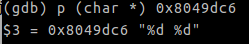
\includegraphics[scale=0.8]{images/phase_3_part_0.png}
	\end{figure}	
	
	“$\%d \%d$”代表读入了两个整数。调用sscanf结束后,将sscanf的返回值与1比较,若不大于1则炸弹爆炸。
	
	由此可以得到我们这关的目标是输入两个整数\textbf{a b}。
	
	\item
	输入的两个整数\textbf{a b}存放在\textbf{0x18($\%$esp)} 和 \textbf{0x1c($\%$esp)}中。接着往下看程序:
		
		
	\lstinputlisting[language={[x86masm]Assembler}]{sources/phase_3_part_1.asm}

	这里可以发现,程序将\textbf{0x18($\%$esp)}, 即输入的第一个整数\textbf{a}与7进行比较,如果大于7则炸弹爆炸。同时,由于使用的是\textbf{ja}命令,即\textbf{a}为无符号数,\textbf{a}应该不小于0
	
	这样我们可以得出第一个限制条件:输入的第一个	整数 $0 \le a \le 7$
	
	继续往下看,注意到这一段:	
	
	\lstinputlisting[language={[x86masm]Assembler}]{sources/phase_3_part_2.asm}

	\item
	这段具有很明显的\textbf{switch}语句的特征,而跳转表存放在\textbf{0x8049a5c}中。
\newpage		
	于是调用gdb,先查看对应的跳转表:	
	\begin{figure}[h]
		\centering
			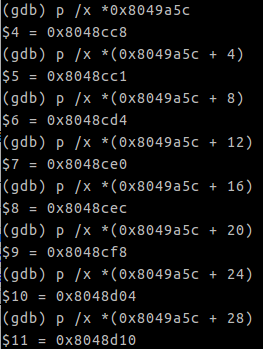
\includegraphics[scale=0.77]{images/phase_3_part_3.png}
	\end{figure}
	
	这样可以将接下来的代码划分模块:	
	
	\lstinputlisting[language={[x86masm]Assembler}]{sources/phase_3_part_4.asm}
	
	\item
	于是可以得出对应的c语言代码:
	
	\lstinputlisting{sources/switch_origin.txt}

	经过整理后的代码如下:
	
	\lstinputlisting{sources/switch.txt}
	
	\item
	在switch语句段后,有这么一段:
	
	\lstinputlisting[language={[x86masm]Assembler}]{sources/phase_3_part_5.asm}
	
	这里给出了第二个限制条件: 输入的第一个整数$a \le 5$
	
	最后,程序将输入的第二个整数\textbf{b}与switch的结果进行比较,不同则炸弹爆炸。
	
	\item
	因此,这关的答案就水落石出了:
		\begin{center}
			输入一个整数$a(0 \le a \le 5)$, 和a经过switch之后的结果b
		\end{center}
	\end{itemize}		
	选用\textbf{a = 4, b = 168},顺利过关

	\begin{figure}[h]
		\centering
			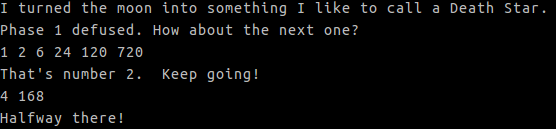
\includegraphics[scale=0.8]{images/phase_3_success.png}
	\end{figure}	